\documentclass{article}

\usepackage[margin=1.0in]{geometry}
\usepackage{graphicx}
\usepackage{amsmath}
\usepackage{float}
\usepackage{enumitem}

\title{CSC 535 HW5}
\date{10/22/2018}
\author{Simon Swenson}

\begin{document}

\pagenumbering{gobble}
\maketitle
\pagenumbering{arabic}

\large Introduction

\small 

\section{Q1}

\begin{figure}[!ht]
	\centering
	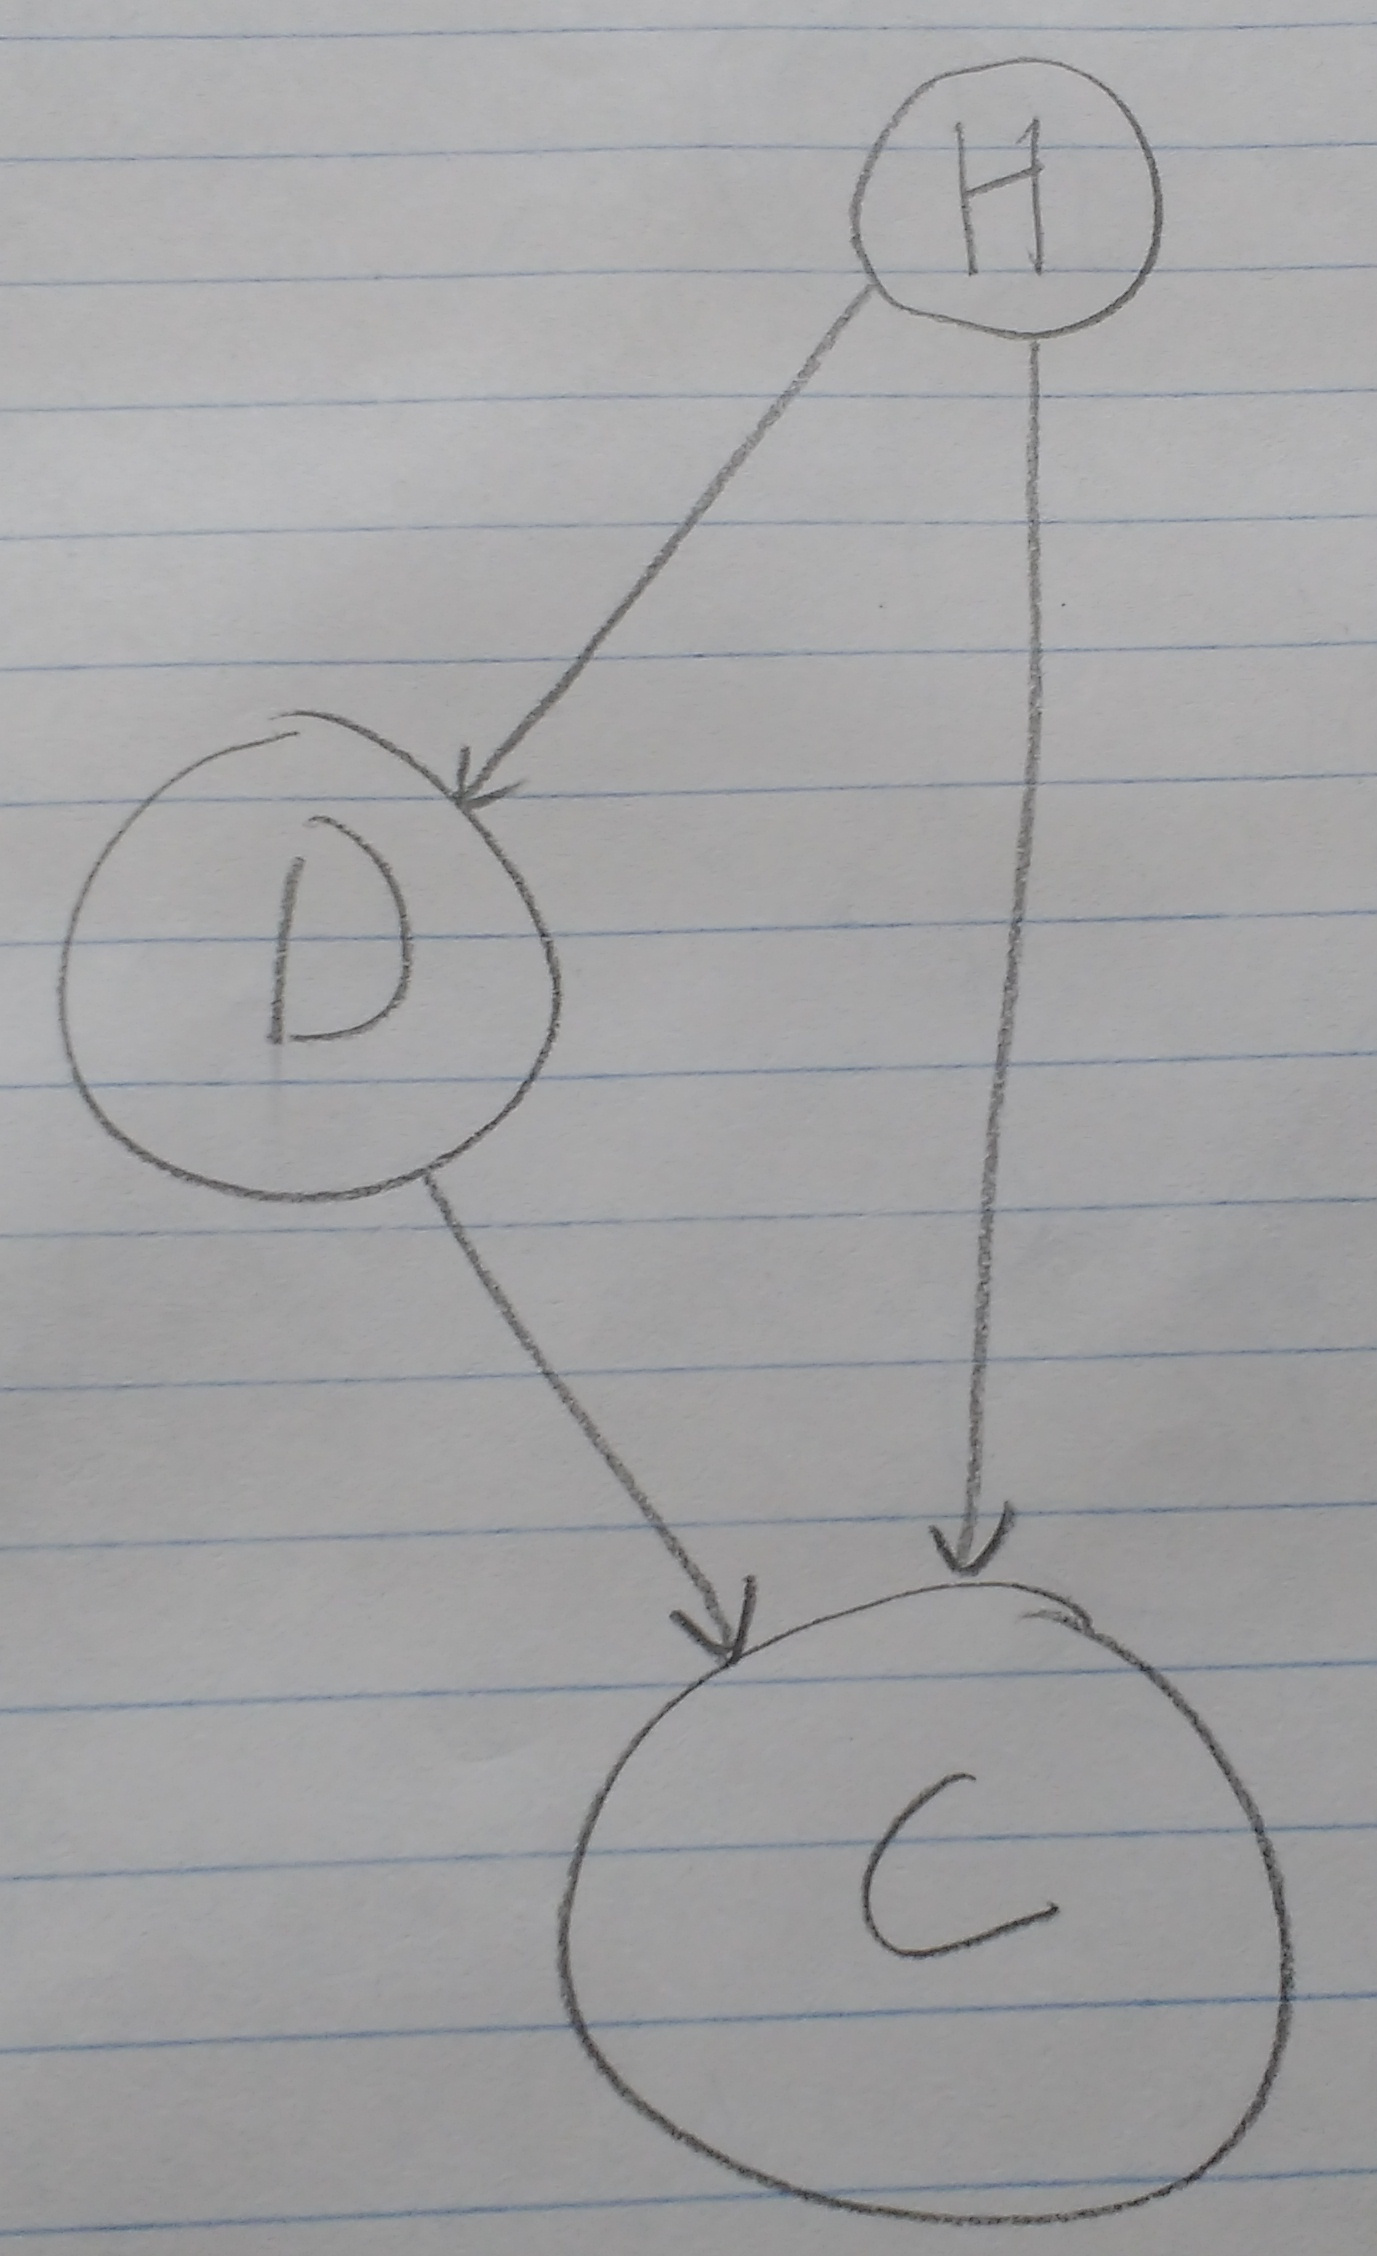
\includegraphics[width=80mm]{figs/drug-bayess-net.jpg}
	\caption{The Bayes's net based on Q1's description.}
\end{figure}

\begin{figure}[!ht]
	\centering
	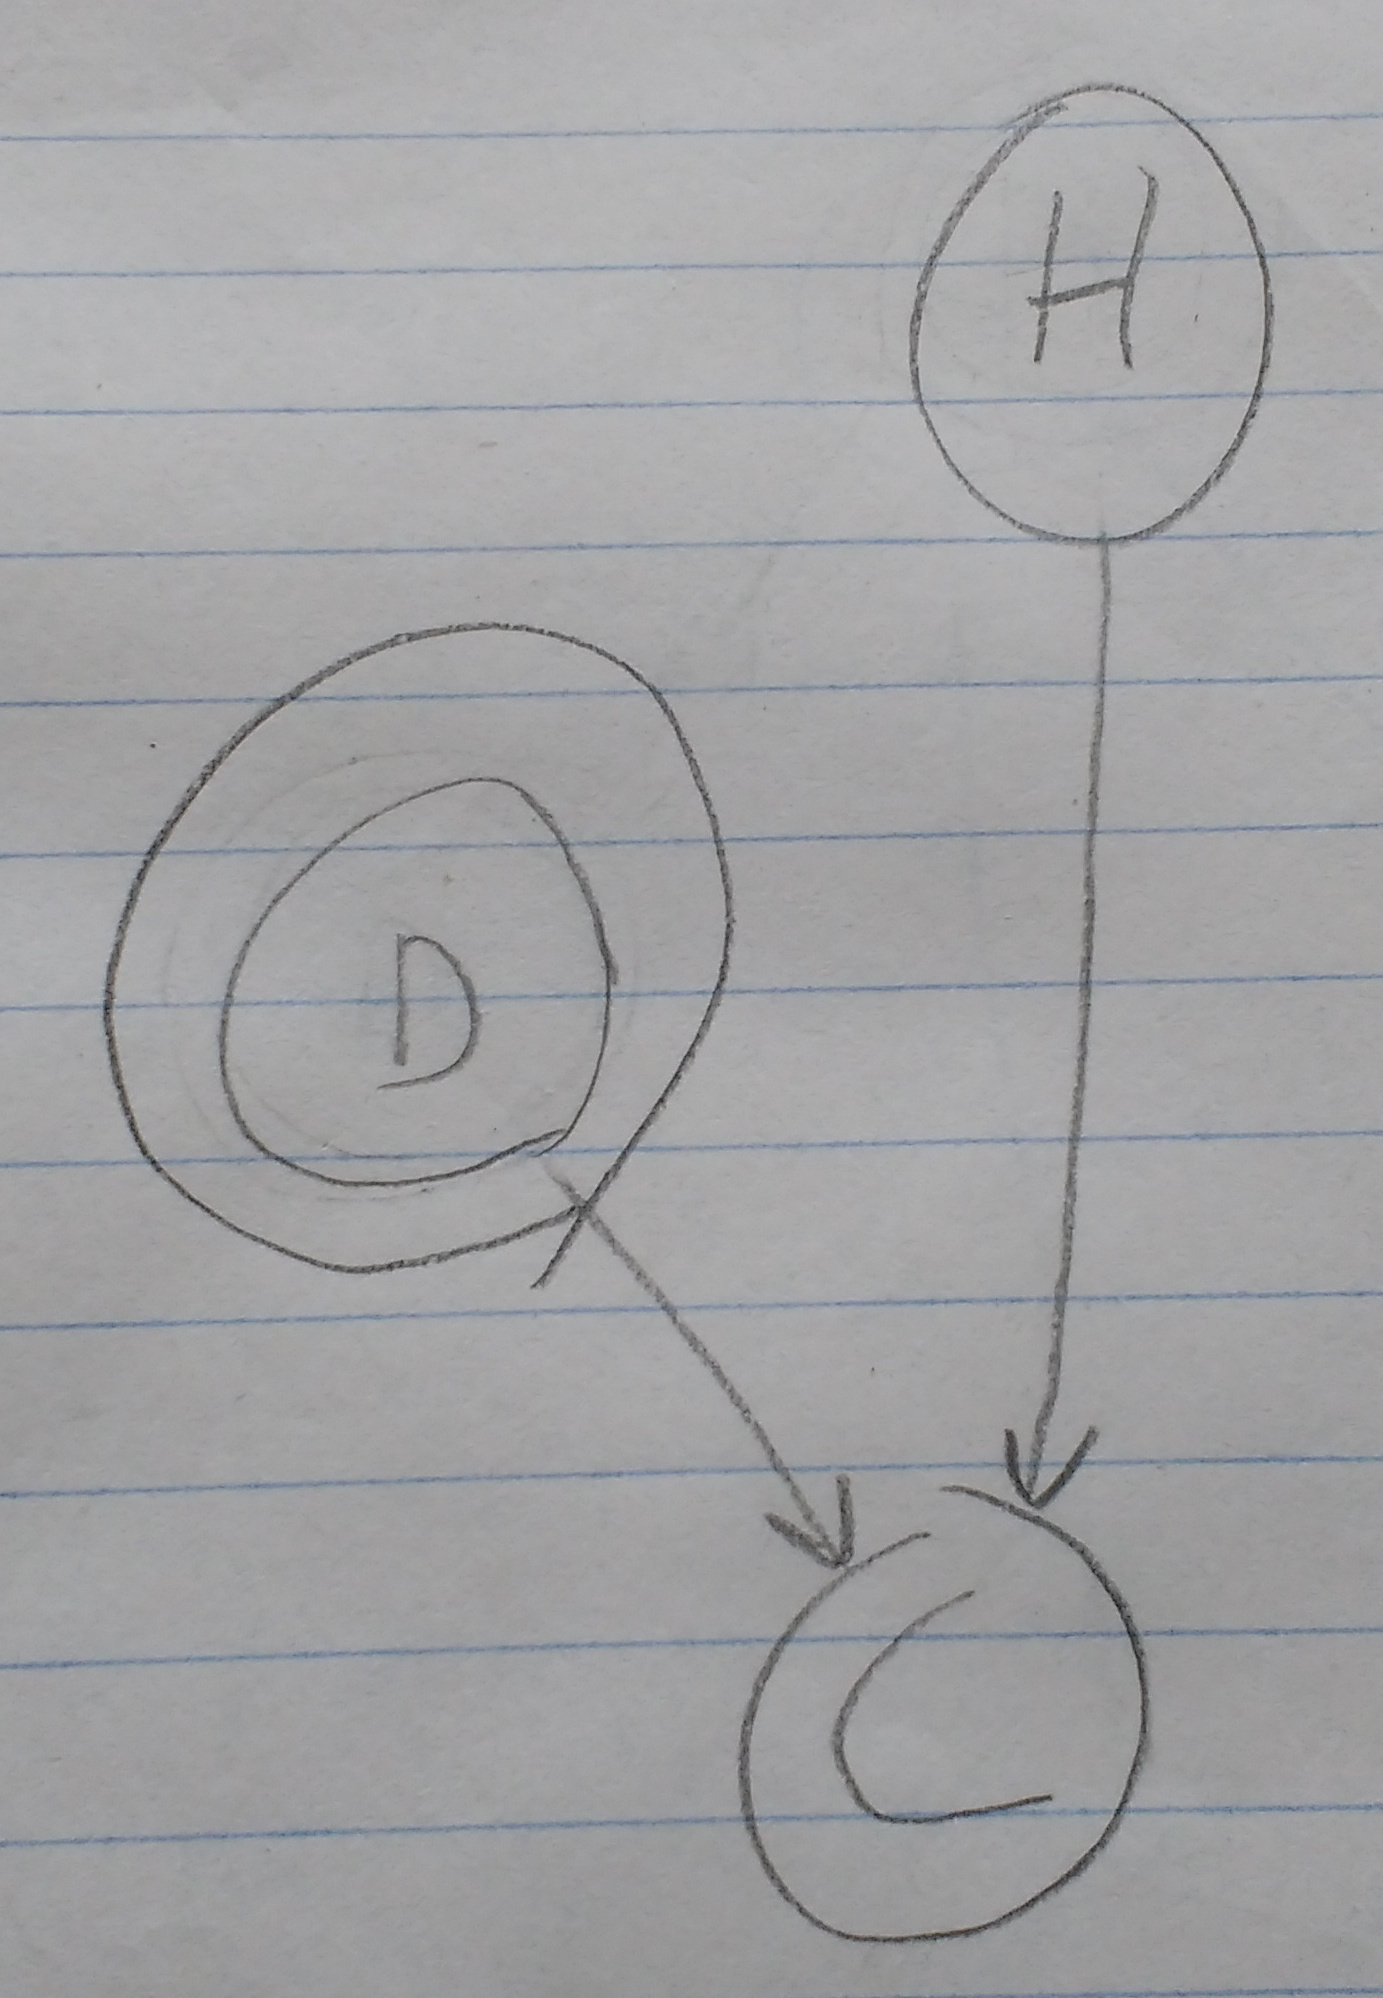
\includegraphics[width=80mm]{figs/drug-bayess-net-experiment.jpg}
	\caption{In terms of intervention, it is impossible to remove the effect 
        of health consciousness from whether the individual was cured or not 
        without also removing the effect of the drug on whether they were cured. 
        However, if we intervene on whether or not they took the drug, we can 
        at least eliminate the connection between H (health conscious) and D 
        (whether they took the drug). Then, we can simply record whether or not 
        they were health conscious. Thus, for each participant, we would know 
        both D and H.}
\end{figure}

The joint distribution chart, representing the first Bayes's net, is below:

\begin{tabular}{c | c c}
          & H = 0 & \\
    \hline \\
          & D = 0 & D = 1 \\
    \hline \\
    C = 0 & 0.324 & 0.042 \\
    C = 1 & 0.216 & 0.018 \\
\end{tabular}

~\\

\begin{tabular}{c | c c}
          & H = 1 & \\
    \hline \\
          & D = 0 & D = 1 \\
    \hline \\
    C = 0 & 0.008 & 0.108 \\
    C = 1 & 0.032 & 0.252 \\
\end{tabular}

Just looking at the numbers, we see that health conscious people tend to take 
the drug much more often than non health conscious people. Based on Example 
21.14 in Bishop's book, we can calculate equations which represent the second 
Bayes's net, $ P(C = 1 | do(D = 0)) $ and $ P(C = 1 | do(D = 1)) $:

\begin{align*}
P(C = 1 | do(D = 1)) &= \sum_H P(C = 1 | D = 1, H) P(H) \\
                    &= P(C = 1 | D = 1, H = 0) P(H = 0) + P(C = 1 | D = 1, H = 1) P(H = 1) \\
                    &= \frac{0.018}{0.042 + 0.018} 0.6 + \frac{0.252}{0.108 + 0.252} 0.4 \\
                    &= (0.3)(0.6) + (0.7)(0.4) \\
                    &= 0.18 + 0.28 \\
                    &= 0.46
\end{align*}

\begin{align*}
P(C = 1 | do(D = 0)) &= \sum_H P(C = 1 | D = 0, H) P(H) \\
                    &= P(C = 1 | D = 0, H = 0) P(H = 0) + P(C = 1 | D = 0, H = 1) P(H = 1) \\
                    &= \frac{0.216}{0.324 + 0.216} 0.6 + \frac{0.032}{0.008 + 0.032} 0.4 \\
                    &= (0.4)(0.6) + (0.8)(0.4) \\
                    &= 0.24 + 0.32 \\
                    &= 0.56
\end{align*}

Running the experiment has demonstrated that, 
though $ P(C = 1 | D = 1) \approx 0.521 > 0.479 \approx P(C = 1 | D = 0)$, 
cures happen more likely when the drug is \textit{not} taken.

\section{Q2}

\subsection{a}

(See next two pages for figures.)

\begin{figure}
	\centering
	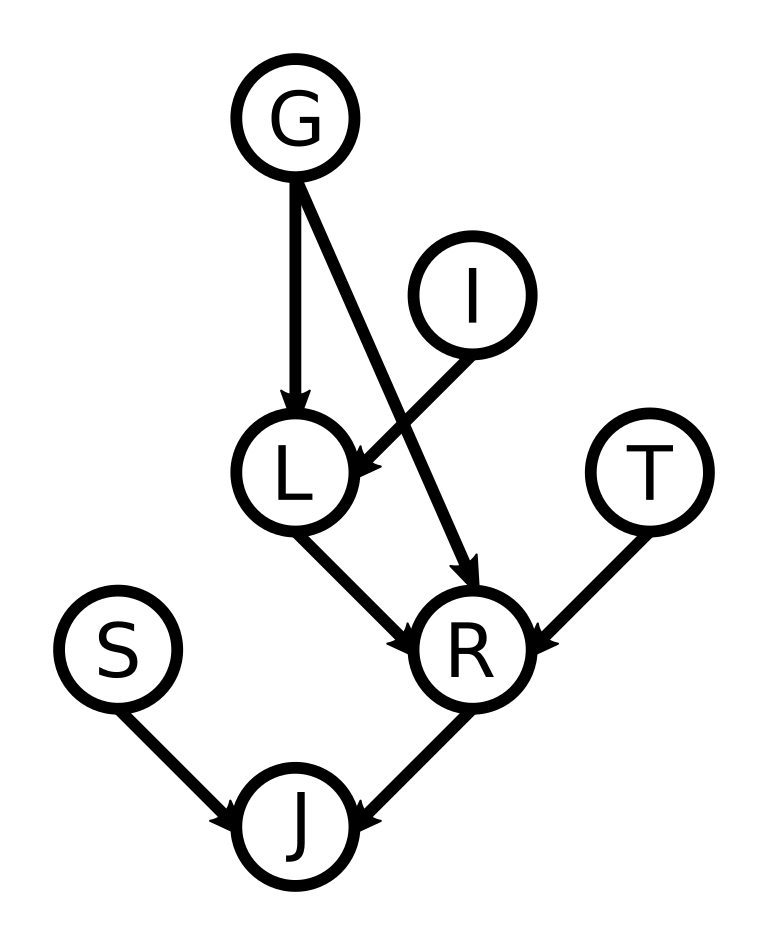
\includegraphics[width=120mm]{figs/education-bayess-net.png}
	\caption{The Bayes's net based for the previous homework assignment, wherein
        factors for success in education and industry are considered.}
\end{figure}

\begin{figure}
	\centering
	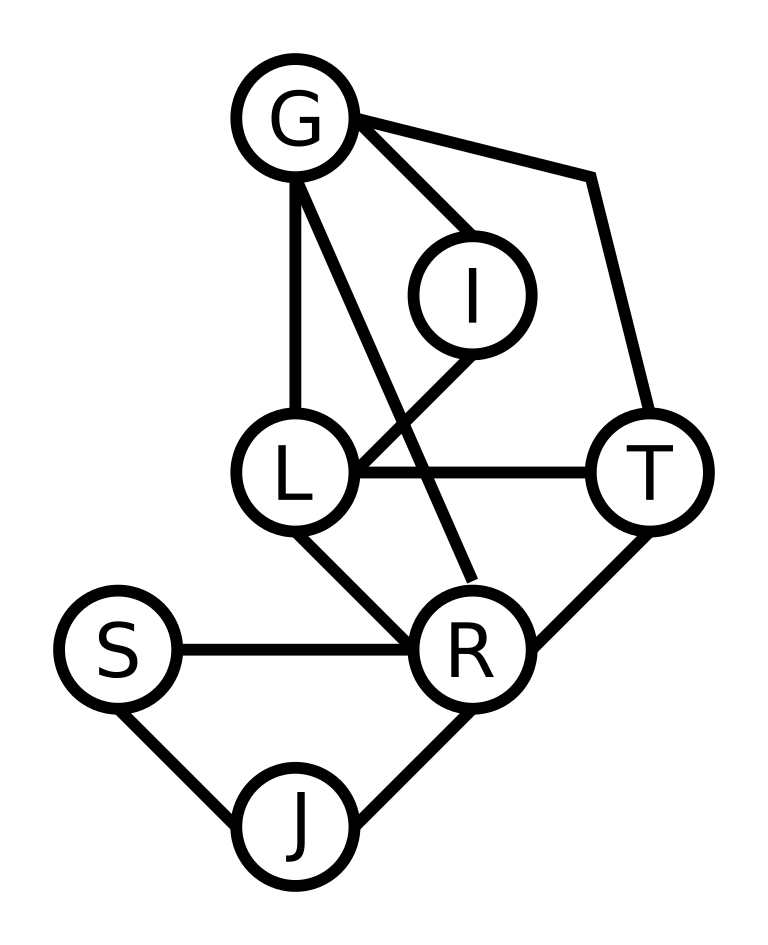
\includegraphics[width=120mm]{figs/education-mrf.png}
	\caption{The Markov random field converted from the previous graph. The 
        main steps involved are to (1) marry parents and (2) remove all arrows.
        In this case, L has two parents, G and I, which must be married. R has 
        three parents, L, T, and G, which must be married. J has two parents, S 
        and R, which must be married. Then, all arrows are simply removed. Doing 
        so loses independence information about the parents. For example, G and 
        I were independent in the Bayes's net, but, now that they are married, 
        they exist in the same clique.}
\end{figure}

~\\
~\\
~\\
~\\
~\\
~\\
~\\
~\\
~\\
~\\
~\\
~\\
~\\
~\\
~\\
~\\
~\\
~\\
~\\
~\\
~\\
~\\
~\\
~\\
~\\
~\\
~\\
~\\


\subsection{b}

Markov random fields are factored in terms of the clique potential/energy. Using 
maximal cliques allows us to use a minimal number of factors. Let's begin 
choosing cliques using a greedy algorithm. Note that above, L, T, and G were 
married. That is a clue that a large clique, $ \{R, L, T, G\} $, exists. I is 
connected to the graph via $ \{G, I\} $ and $ \{I, L\} $. Finally, we have the 
clique $\{J, R, S\}$.

Note that converting a Bayes's net distribution to Markov random 
field clique potentials is not unique. Let's factor in the 
following way:

\begin{align*}
\psi_{G, L, R, T}(G, L, R, T) &= P(G) P(L | G) P(T) P(R | G, L, T) \\
\psi_{G, I}(G, I) &= 1 \\
\psi_{I, L}(I, L) &= P(I) \\
\psi_{J, R, S}(J, R, S) &= P(S) P(J | R, S)
\end{align*}

\section{Q3}

\subsection{a}

(See next page for figure.)

\begin{figure}[!ht]
	\centering
	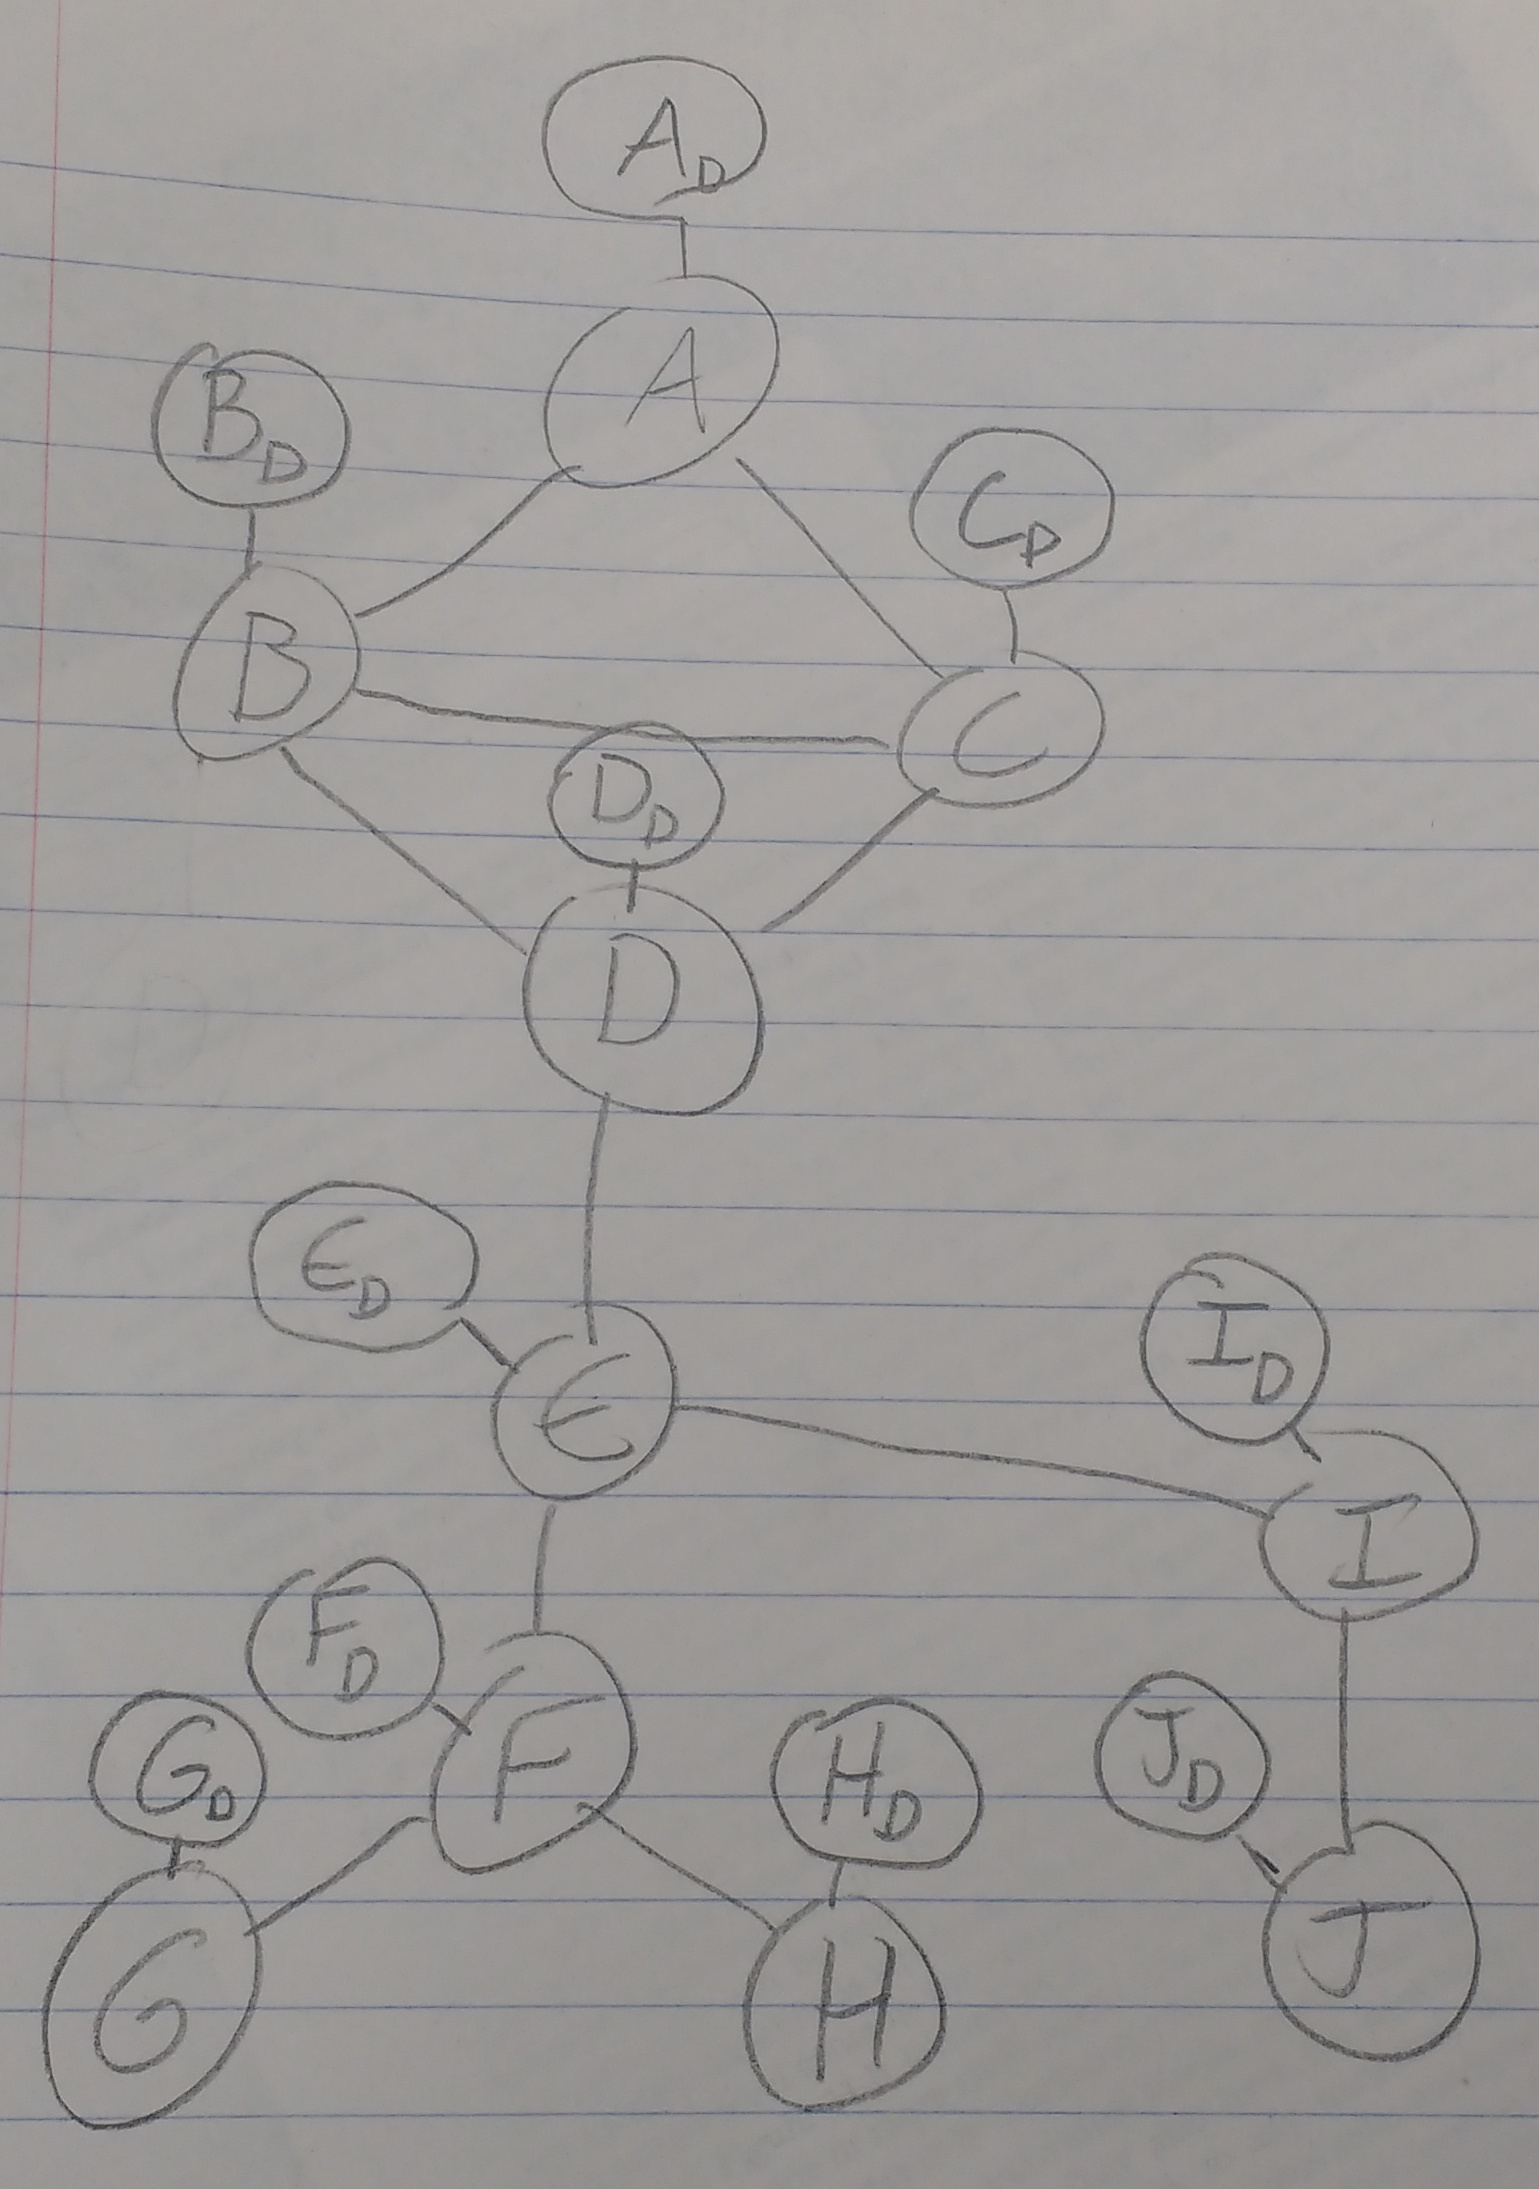
\includegraphics[width=120mm]{figs/friendship-mrf.jpg}
	\caption{The Markov random field for a group of ten students.
        Each "normal" node represents what operating system that student 
        prefers, and the subscripted Ds represent our observations 
        of those students' operating system choices.}
\end{figure}

~\\
~\\
~\\
~\\
~\\
~\\
~\\
~\\
~\\
~\\
~\\
~\\
~\\
~\\
~\\
~\\
~\\
~\\
~\\
~\\
~\\
~\\
~\\
~\\
~\\
~\\
~\\
~\\
~\\
~\\
~\\
~\\
~\\
~\\
~\\
~\\
~\\
~\\
~\\
~\\
~\\

\subsection{b}

\begin{align*}
\{A_D, A\} \\
\{B_D, B\} \\
\{C_D, C\} \\
\{A, B, C\} \\
\{D_D, D\} \\
\{B, C, D\} \\
\{E_D, E\} \\
\{D, E\} \\
\{F_D, F\} \\
\{E, F\} \\
\{G_D, G\} \\
\{F, G\} \\
\{H_D, H\} \\
\{F, H\} \\
\{I_D, I\} \\
\{E, I\} \\
\{J_D, J\} \\
\{I, J\}
\end{align*}

\subsection{c}

\begin{align*}
& P(A, A_D, B, B_D, C, C_D, D, D_D, E, E_D, F, F_D, G, G_D, H, H_D, I, I_D, J, J_D) = \\
& \psi_{A, A_D} \psi_{B, B_D} \psi_{C, C_D} \psi_{A, B, C} \psi_{D, D_D} \psi_{B, C, D} \\
& \psi_{E, E_D} \psi_{D, E} \psi_{F, F_D} \psi_{E, F} \psi_{G, G_D} \psi_{F, G} \\
& \psi_{H, H_D} \psi_{F, H} \psi_{I, I_D} \psi_{E, I} \psi_{J, J_D} \psi_{I, J}
\end{align*}

\subsection{d}

Recall that conditioning on a node blocks paths that go through that node. That is 
the only way that paths are blocked in a Markov random field. Thus, A is not 
independent of J.

\subsection{e}

Though conditioning on C blocks one potential path from A to D, there is still 
an unblocked path through B, so the A and D remain dependent, conditioned on C.

\subsection{f}

Yes, A and E are independent conditioned on D. All paths from A to E must pass 
through D, so conditioning on D blocks all such paths.

\subsection{g}

Recall that energy is inversely proportional to probability. Thus, to make 
something more likely, energy must be removed. Such an energy factor for this 
question must have several factors: (1) a constant factor bias toward macs, (2) 
a factor that accounts for, for each neighbor, that neighbor having a mac 
increases your chances of having a mac, (3) the count of macs in a given clique 
must be less than 3, and (4) Detector output is correlated with actual 
preference. Given these factors, let us construct a corresponding energy function. 
Let $x$ be the set of non-observation nodes in the Markov random field and $y$ 
be the set of observation nodes. Let $ C_x $ be the set of cliques which 
contain only non-observation nodes.

First, the constant term is easy: $-|x| \alpha$, so a higher preference constant results 
in a lower energy, which results in a higher probability. We multiply that by 
the number of students.

Second, a factor which decreases as neighbor similarity increases would be the 
sum over neighbors of the multiple of the neighbor values: 
$-\beta \sum_{x_i, x_j | neighbors(x_i, x_j) \wedge mac(x_j) } 1$.

Third, to ensure that no clique ever has more than two mac users, we can 
construct a piecewise energy function with energy equal to infinity if any 
clique has more than two mac users.

Last, a factor which decreases as detector output and actual preference is correlated is: $-\gamma \sum_i x_i y_i$

$$
E(x, y) =
\begin{cases}
    \infty & \sum_{c \in C_x | MoreThanTwoMacUsers(c)} 1 > 0 \\
    -|x| \alpha - \beta \sum_{i, j | Neighbors(x_i, x_j) \wedge Mac(x_j) } 1 - \gamma \sum_i x_i y_i & otherwise
\end{cases}
$$

\section{Q4}

\subsection{a}

I think this is very similar to the example from class with a random, noisy 
image. Thus, my approach to constructing a MRF given the problem statement is 
to create a node for each region. That node would represent the ground truth of 
the region's label. Then, that node would have 
a connecting node representing p(noun, region-features) for that particular 
region. Energy would relate those two nodes together. Furthermore, since 
adjacent regions are more likely to be the same noun, we would have an energy 
factor relating adjacent region nodes. Here is a MRF for it:

\begin{figure}[!ht]
	\centering
	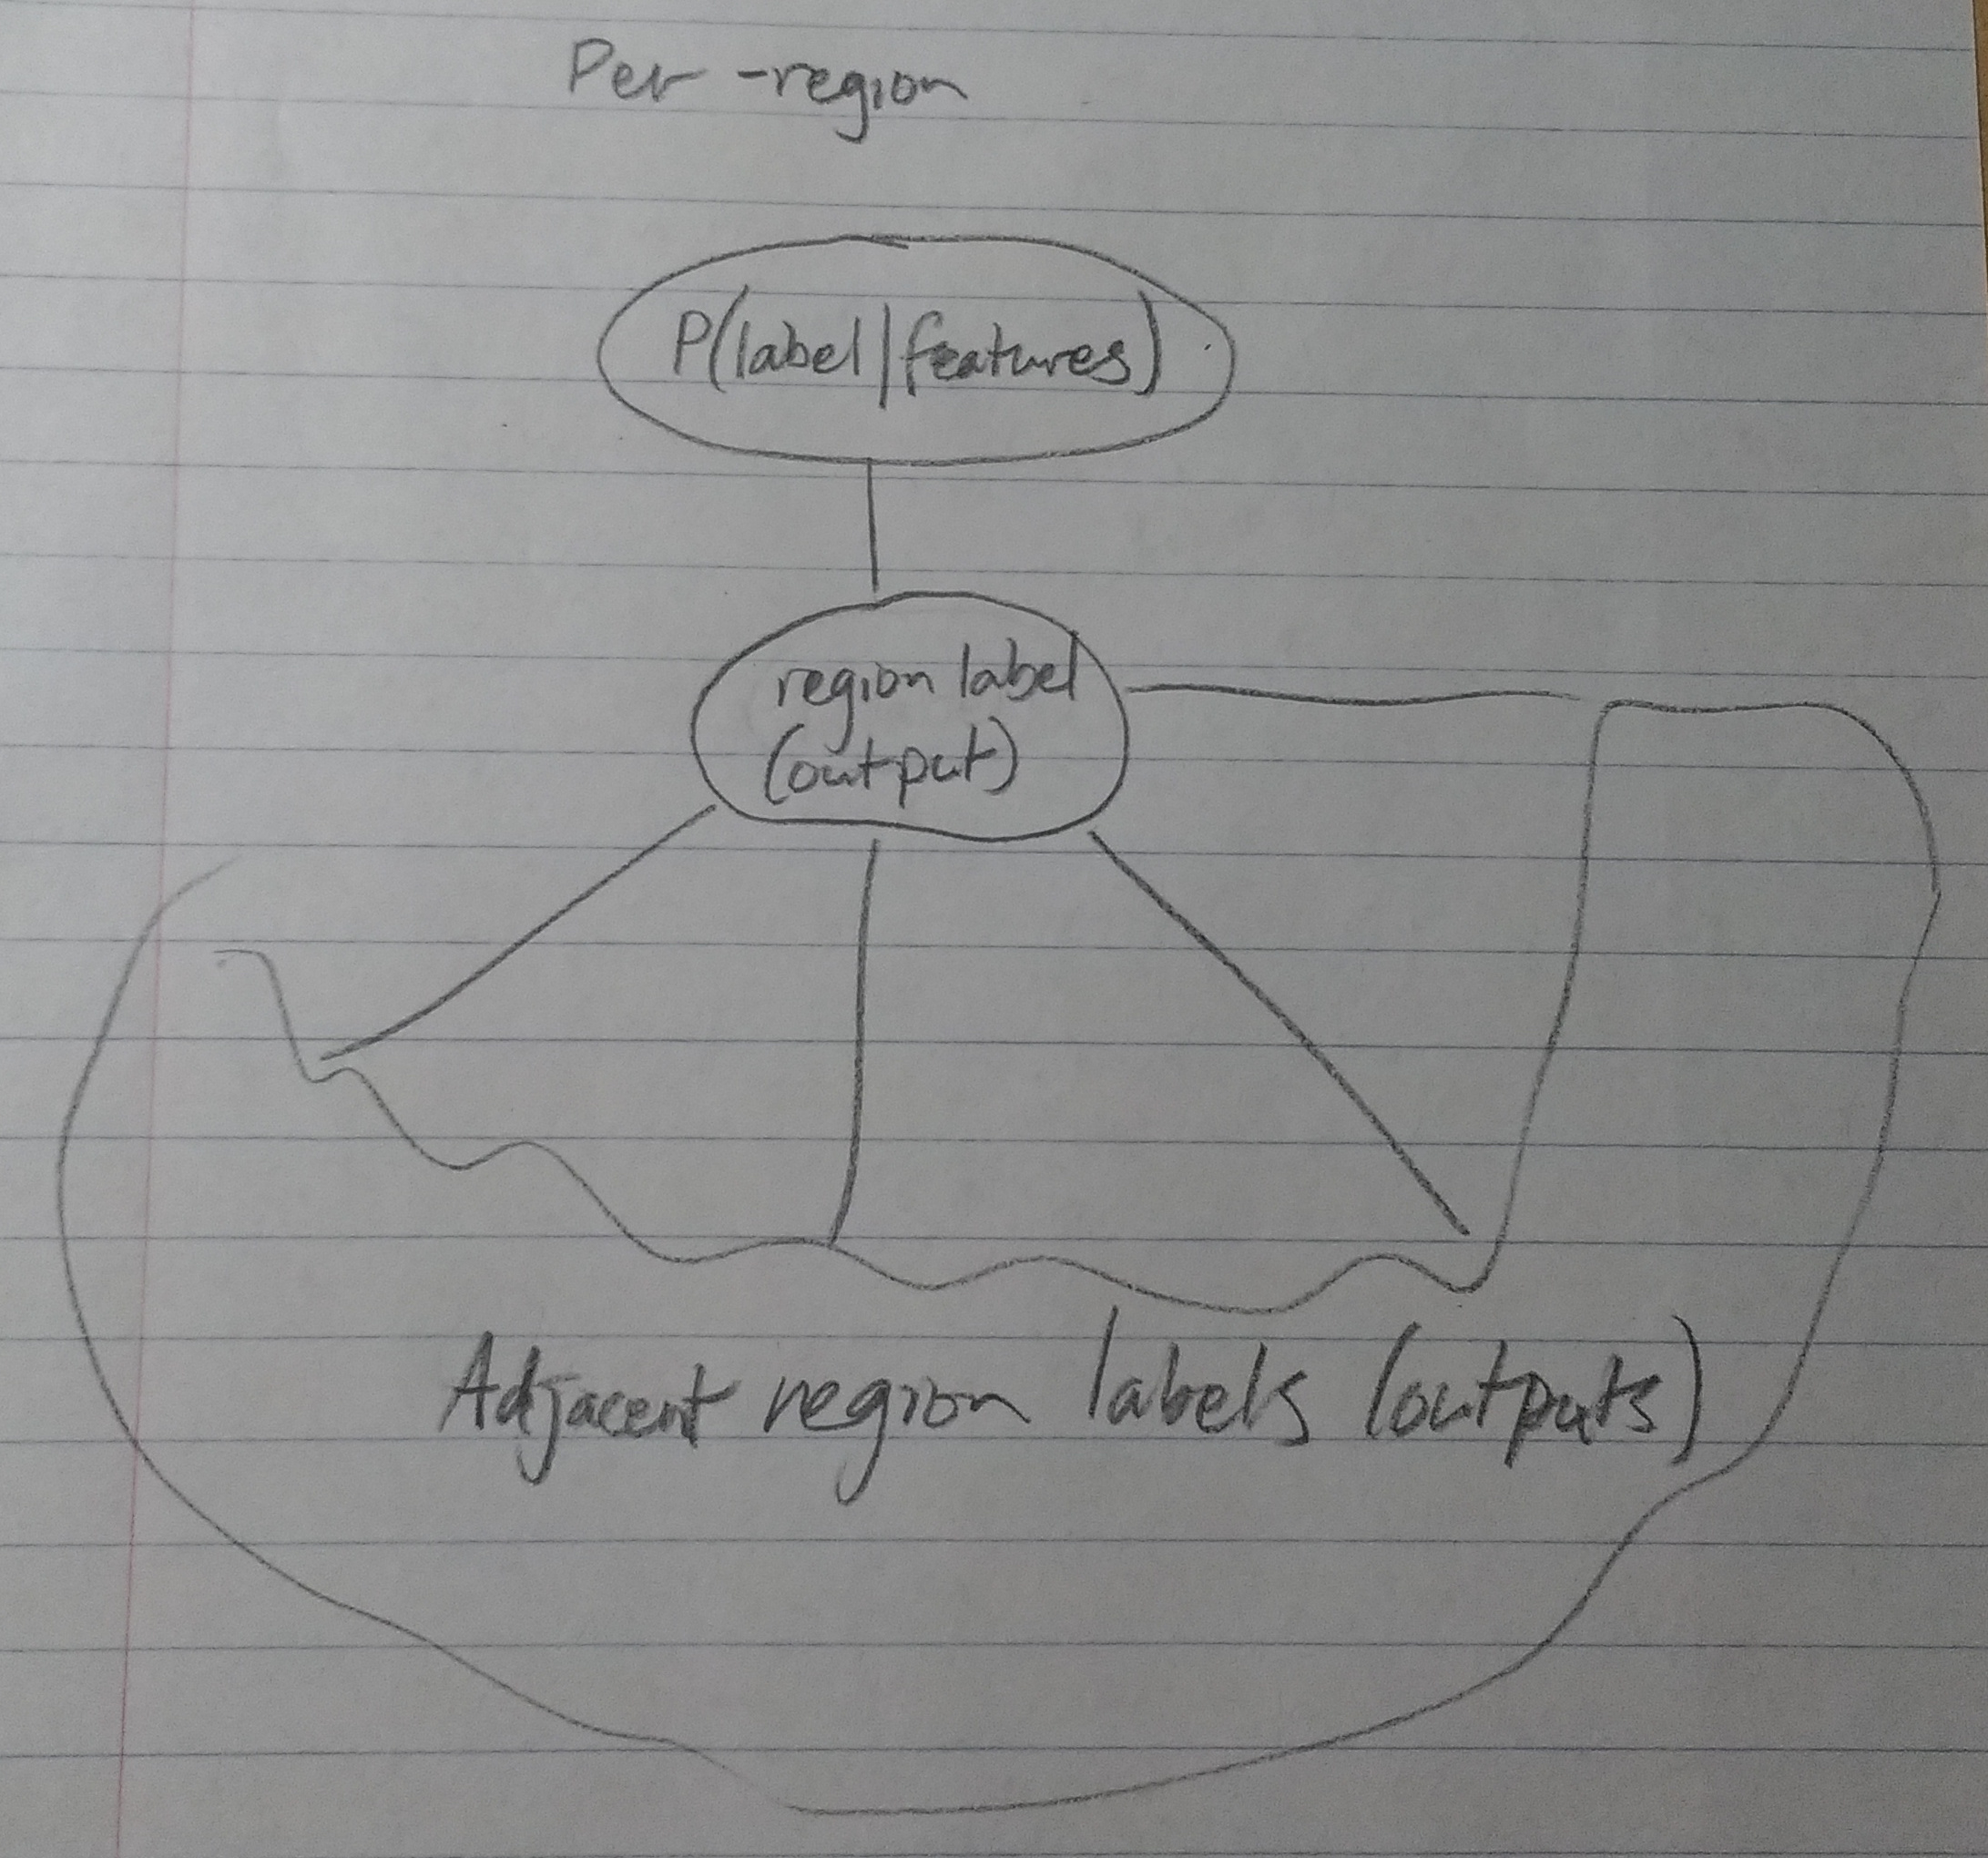
\includegraphics[width=120mm]{figs/region-by-noun-mrf.jpg}
	\caption{The Markov random field for determining the best label for a 
        region. Such a label is related to the naive label, given only the 
        region's features, and the best label for adjacent regions.}
\end{figure}

The probability function can be given as:

\begin{align*}
P &= \frac{1}{Z} \prod_{c \in C} \psi_c \\
 &= \frac{1}{Z} e^{-E(x)}
\end{align*}

Now, we only need to define an energy function. I've already mentioned that, for 
each region, it should relate the corresponding naive label, given only the 
region's features, and the best label for each adjacent region. Here is one 
such expression:

$$
E = - \alpha \sum_{i, j | Neighbors(x_i, x_j)} x_i x_j - \beta \sum_{i} x_i y_i
$$

Just substitute E into the equation above to get the corresponding probability.

Random assignments of labels allows us to compute the energy for that particular 
instance and thus the probability.

\subsection{b}

Here, we could add an additional node between each region, which represents the 
probability that a (preposition, noun, noun) tuple fits the given link. If we 
wanted to simplify our model, we could enforce that only adjacent regions can 
have connecting prepositions. Here's the corresponding MRF:

\begin{figure}[!ht]
	\centering
	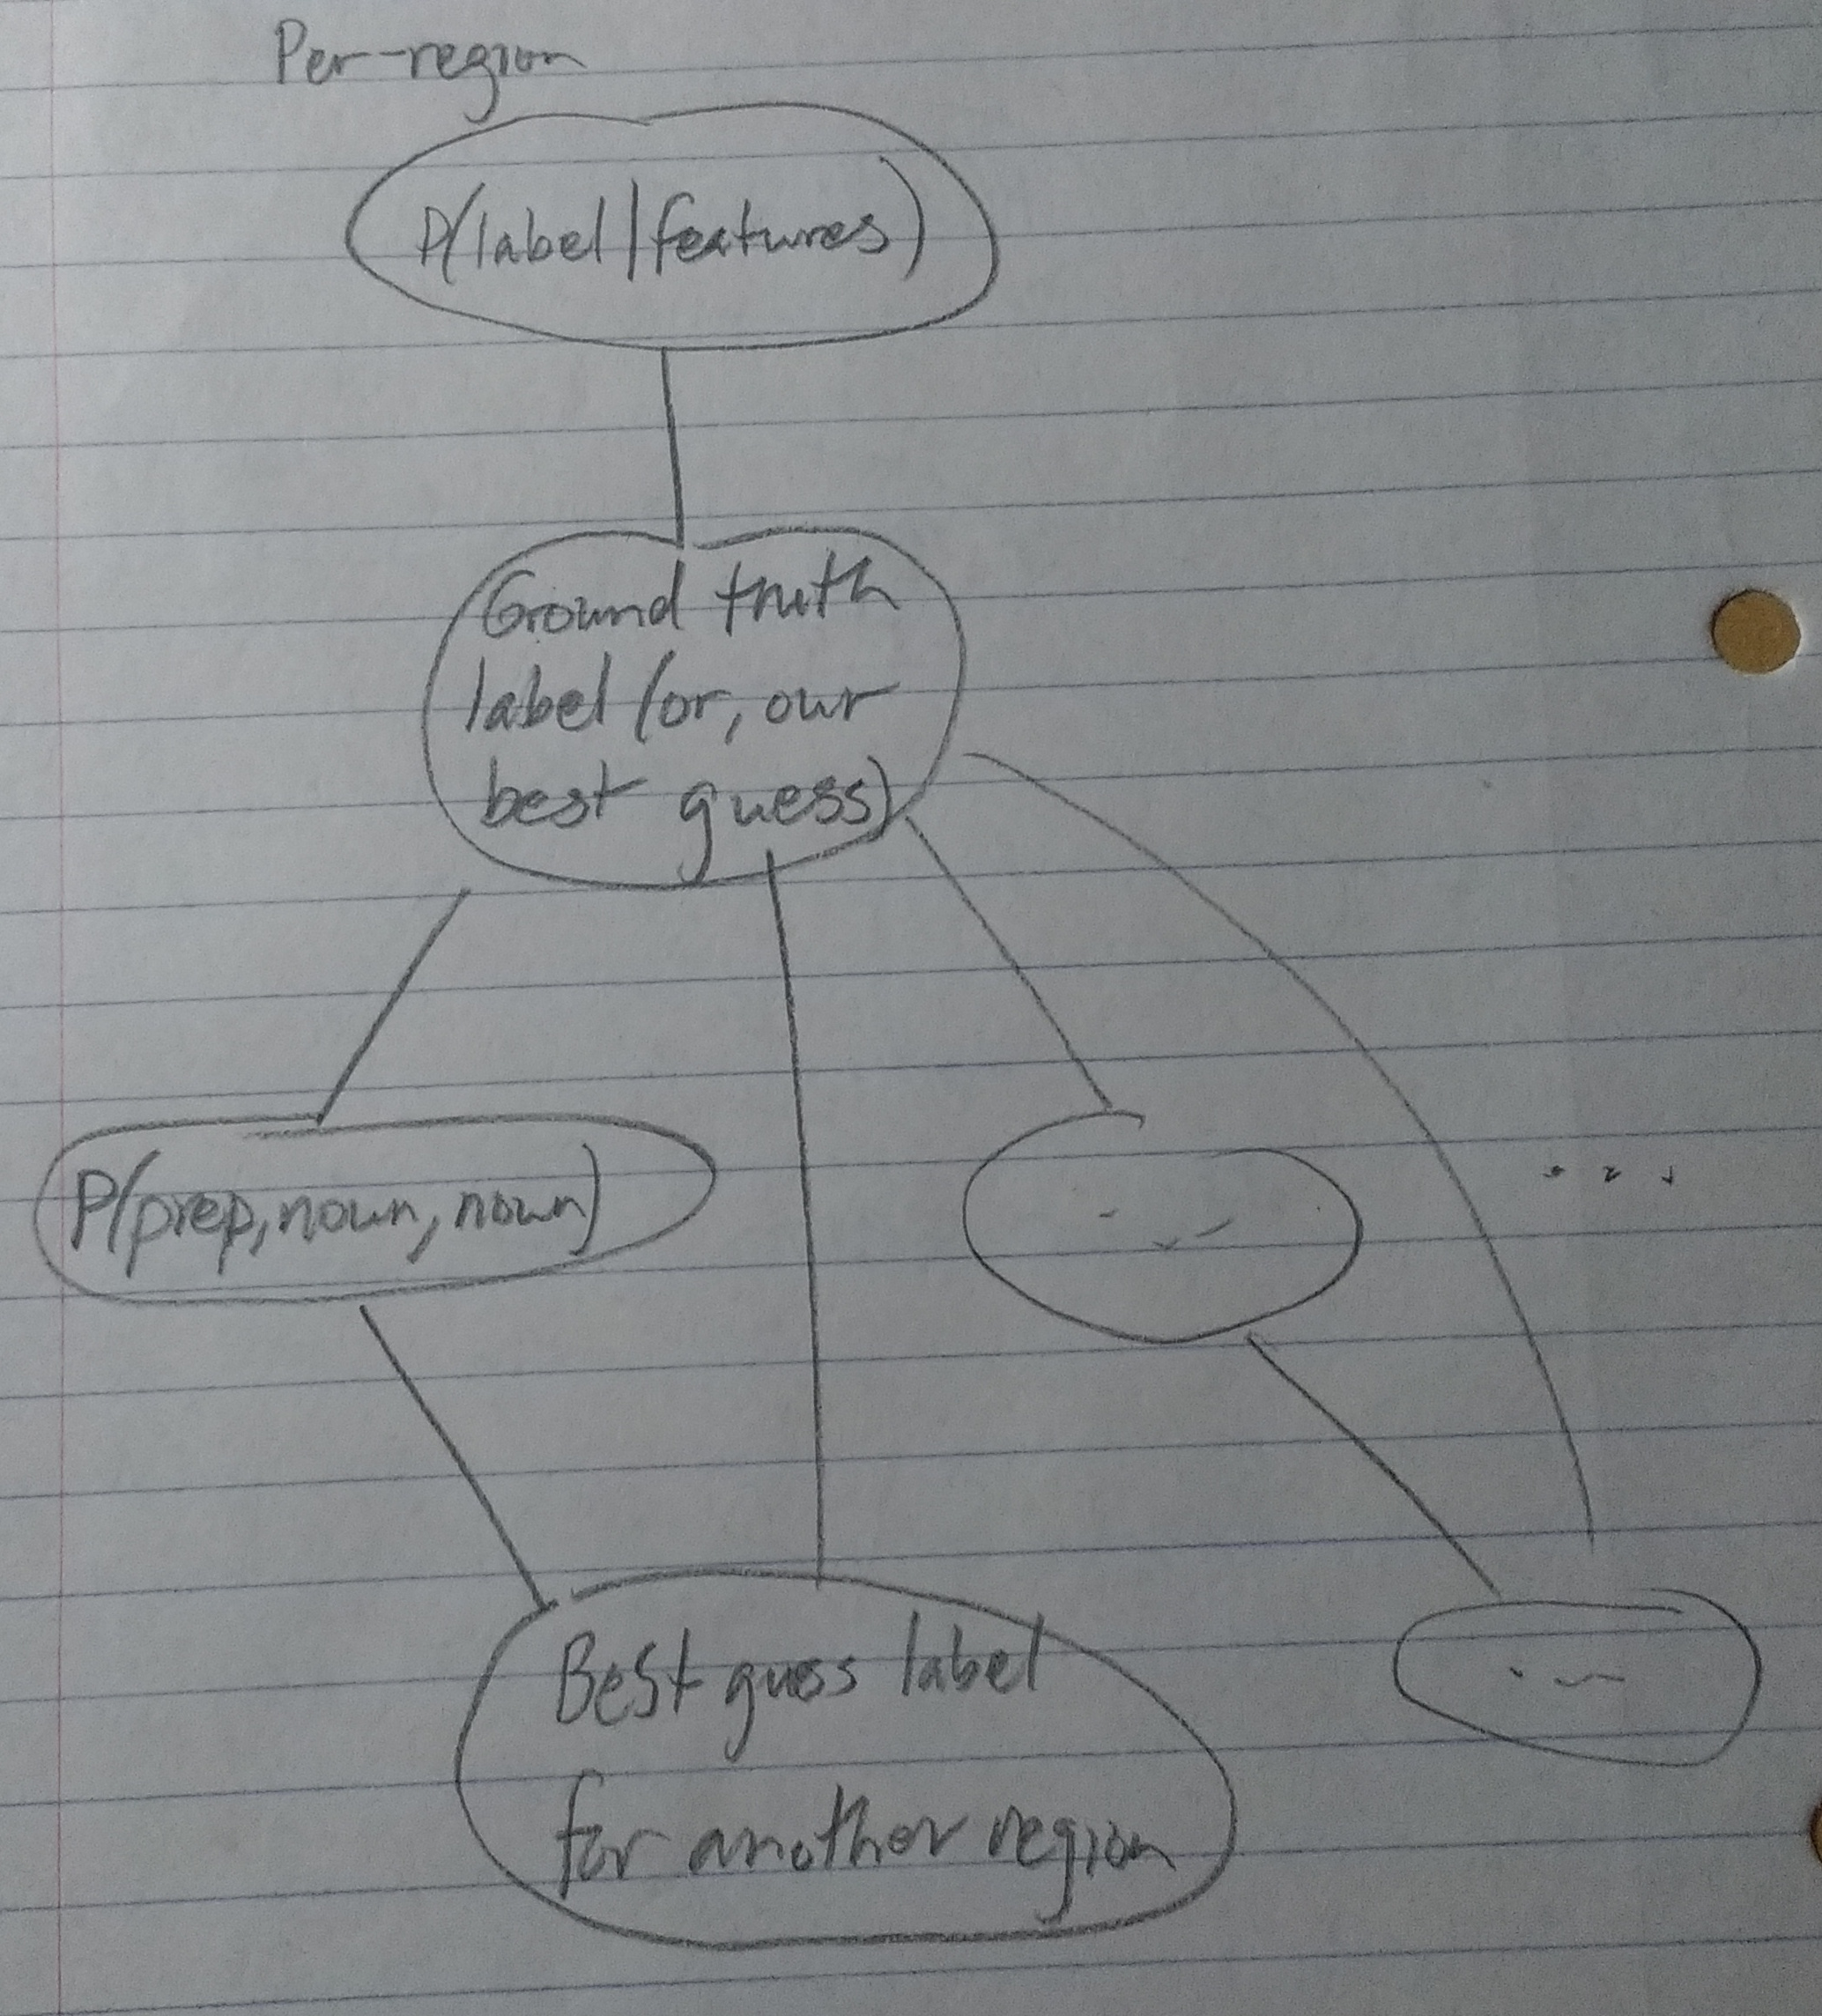
\includegraphics[width=120mm]{figs/region-by-noun-and-prep-mrf.jpg}
	\caption{The Markov random field for determining the best label for a 
        region. Such a label is related to the naive label, given only the 
        region's features, and the best label for adjacent regions.}
\end{figure}

We can slightly tweak the energy function to handle the additional nodes:

$$
E = - \alpha \sum_{i, j | Neighbors(x_i, x_j)} x_i x_j - \beta \sum_{i} x_i y_i - \gamma \sum_{i, j, prep | Neighbors(x_i, x_j) \wedge prep \in Preps} x_i x_j prep
$$

\end{document}